\documentclass[aspectratio=169]{beamer}

\usetheme{metropolis}
\usepackage{graphicx}
\usepackage{amsmath}
\usepackage{booktabs}
\usepackage{listings}
\usepackage{xcolor}
\usepackage{tikz}

% RE Branding Colors
\definecolor{regreen}{HTML}{1B5E20}
\definecolor{regreenlight}{HTML}{2E7D32}
\definecolor{rewhite}{HTML}{FFFFFF}
\definecolor{regray}{HTML}{4A4A4A}

% Apply RE colors to metropolis theme
\setbeamercolor{palette primary}{bg=regreen, fg=rewhite}
\setbeamercolor{frametitle}{bg=regreen, fg=rewhite}
\setbeamercolor{title separator}{fg=regreenlight}
\setbeamercolor{progress bar}{fg=regreenlight, bg=regreen!20}
\setbeamercolor{alerted text}{fg=regreenlight}
\setbeamercolor{block title}{bg=regreen, fg=rewhite}
\setbeamercolor{block body}{bg=regreen!5}

\lstset{
    basicstyle=\ttfamily\small,
    keywordstyle=\color{regreen},
    stringstyle=\color{red!60!black},
    frame=none,
    breaklines=true,
}

% Logo in footer
\setbeamertemplate{frame footer}{\hfill
\includegraphics[height=0.6cm]{figures/re_logo.jpg}}

\title{Teaching a Tiny Model Arithmetic via RL}
\subtitle{GRPO Fine-Tuning of LFM2-350M}
\author{Wes Griffin}
\institute{Advanced Machine Learning \textemdash{} Ransom Everglades School}
\date{April 2026}

\begin{document}

% ---- TITLE SLIDE ----
{
\setbeamertemplate{frame footer}{}
\setbeamercolor{background canvas}{bg=white}
\begin{frame}[plain]
    \centering
    \vspace{1cm}
    
\includegraphics[width=2cm]{figures/re_logo.jpg}\\[0.5cm]
    {\color{regreen}\rule{0.8\textwidth}{1.5pt}}\\[0.5cm]
    {\Large\color{regreen}\textbf{Teaching a Tiny Model Arithmetic\\via Reinforcement Learning}}\\[0.4cm]
    {\normalsize\color{regray} GRPO Fine-Tuning of LFM2-350M}\\[0.8cm]
    {\small\color{black} Wes Griffin}\\[0.2cm]
    {\footnotesize\color{regray} Advanced Machine Learning \textemdash{} Ransom Everglades School}\\[0.2cm]
    {\footnotesize\color{regray} April 2026}\\[0.5cm]
    {\color{regreen}\rule{0.8\textwidth}{1.5pt}}
\end{frame}
}

% ---- SLIDE 1: Problem ----
\begin{frame}{The Problem}
    \begin{columns}
        \column{0.5\textwidth}
        \textbf{Task:} Given a target number, generate a math expression that evaluates to it.

        \vspace{1em}
        \begin{tabular}{cl}
            \textbf{Target} & \textbf{Valid Output} \\
            \midrule
            7 & \texttt{3 + 4} \\
            73 & \texttt{9 * 8 + 1} \\
            256 & \texttt{16 * 16} \\
            5000 & \texttt{50 * 100} \\
        \end{tabular}

        \column{0.5\textwidth}
        \textbf{Why this task?}
        \begin{itemize}
            \item Perfectly verifiable reward
            \item Requires compositional reasoning
            \item Multiple valid solutions
            \item Difficulty scales naturally
        \end{itemize}
    \end{columns}
\end{frame}

% ---- SLIDE 2: Model ----
\begin{frame}{The Model: LFM2-350M}
    \begin{columns}
        \column{0.55\textwidth}
        \textbf{Liquid AI's LFM2-350M}
        \begin{itemize}
            \item 354M parameters
            \item \alert{Not a transformer} --- hybrid architecture
            \item 10 convolutional + 6 attention layers
            \item Trained on 10T tokens
            \item Designed for edge/on-device AI
        \end{itemize}

        \vspace{0.5em}
        \textit{``We recommend fine-tuning LFM2 on narrow use cases to maximize performance.''}

        \column{0.45\textwidth}
        \centering
        \begin{tabular}{ll}
            \toprule
            Params & 354M \\
            Layers & 16 \\
            Context & 32K \\
            Vocab & 65K \\
            Precision & bf16 \\
            \bottomrule
        \end{tabular}
    \end{columns}
\end{frame}

% ---- SLIDE 3: Method ----
\begin{frame}{Method: GRPO + LoRA}
    \textbf{Group Relative Policy Optimization} (DeepSeekMath, 2024)

    \begin{enumerate}
        \item Generate $G = 8$ completions per prompt
        \item Score each with reward function: $\text{eval}(e) = n$ ?
        \item Compute group-relative advantage: $\hat{A}_i = \frac{r_i - \text{mean}(\mathbf{r})}{\text{std}(\mathbf{r})}$
        \item Update policy with clipped surrogate loss
    \end{enumerate}

    \vspace{1em}
    \textbf{LoRA} fine-tuning: rank 32, targeting attention + MLP layers

    \vspace{0.5em}
    $\rightarrow$ Trains $\sim$2--3\% of parameters. No reward model needed.
\end{frame}

% ---- SLIDE 4: Reward Design ----
\begin{frame}{Reward Design}
    \begin{columns}
        \column{0.55\textwidth}
        \begin{table}
            \centering
            \small
            \begin{tabular}{llc}
                \toprule
                \textbf{Component} & \textbf{What} & \textbf{Wt} \\
                \midrule
                Correctness & eval(expr) == target & 2.0 \\
                Closeness & $1 - |r - n|/|n|$ & 0.5 \\
                Format & \texttt{<expr>} tags & 0.3 \\
                Complexity & Multi-operator bonus & 0.2 \\
                \bottomrule
            \end{tabular}
        \end{table}

        \vspace{0.5em}
        \textbf{Key insight:} Closeness reward prevents sparse gradients early in training.

        \column{0.45\textwidth}
        \centering
        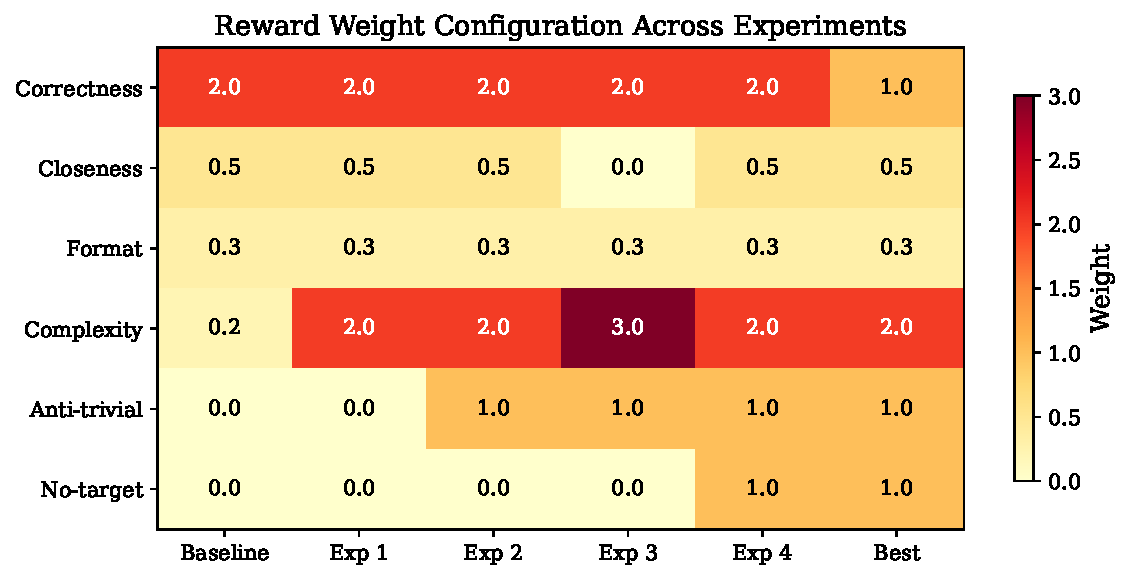
\includegraphics[width=\textwidth]{figures/reward_heatmap.pdf}
    \end{columns}
\end{frame}

% ---- SLIDE 5: Data ----
\begin{frame}{Training Data}
    \begin{columns}
        \column{0.5\textwidth}
        \textbf{10,000 training examples}

        Curriculum distribution:
        \begin{itemize}
            \item 40\% Easy (1--100)
            \item 35\% Medium (100--999)
            \item 25\% Hard (1000--9999)
        \end{itemize}

        \vspace{0.5em}
        Overweight easy targets for initial signal.

        \column{0.5\textwidth}
        \centering
        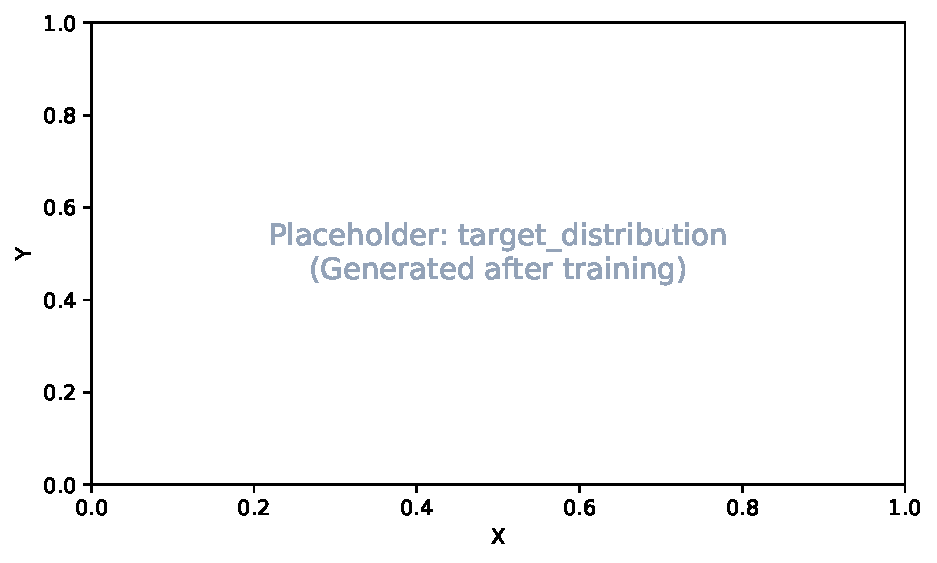
\includegraphics[width=\textwidth]{figures/target_distribution.pdf}
    \end{columns}
\end{frame}

% ---- SLIDE 6: Training Dynamics ----
\begin{frame}{Training Dynamics}
    \begin{columns}
        \column{0.55\textwidth}
        \centering
        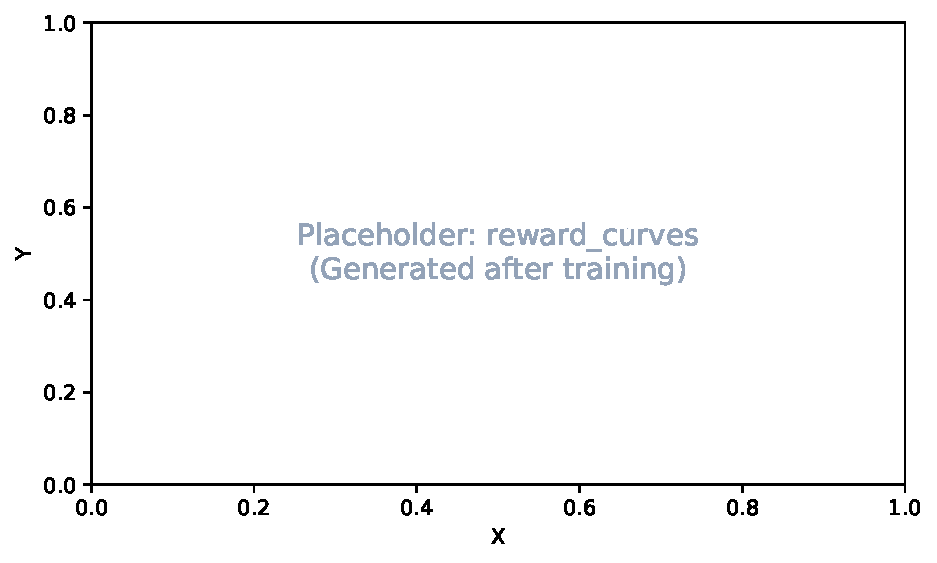
\includegraphics[width=\textwidth]{figures/reward_curves.pdf}

        \column{0.45\textwidth}
        \centering
        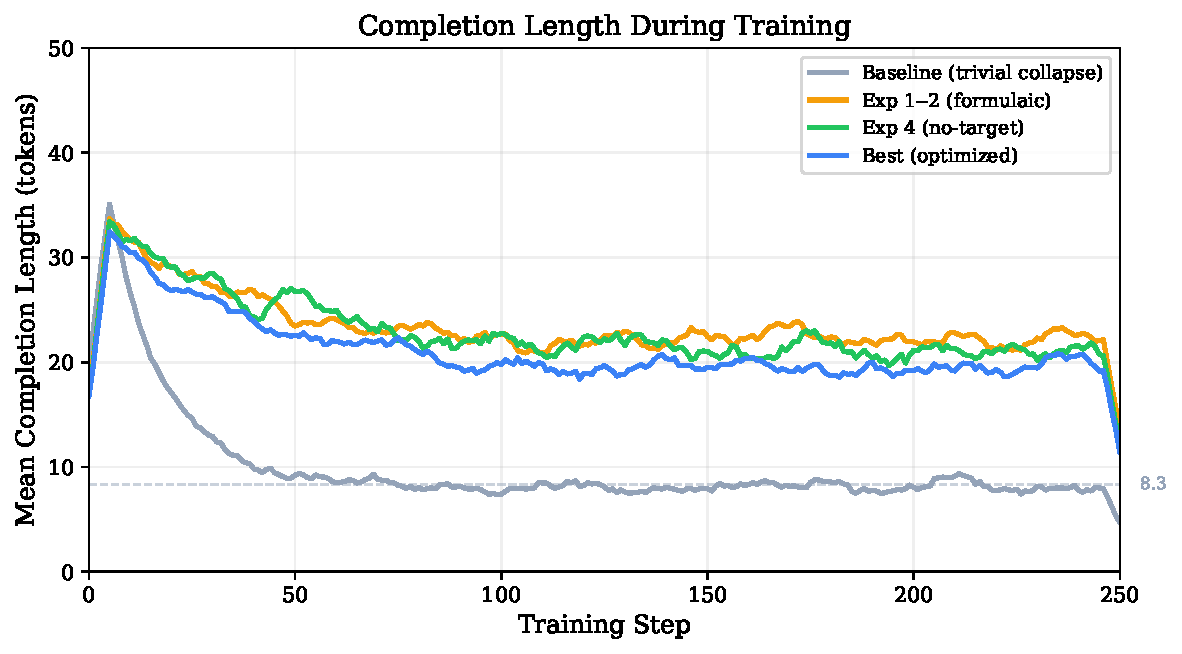
\includegraphics[width=\textwidth]{figures/completion_length.pdf}
    \end{columns}

    \vspace{0.5em}
    \centering
    \small 13 experiments across 2 waves. Baseline collapses to 8 tokens (trivial echo).
\end{frame}

% ---- SLIDE 7: Results Table ----
\begin{frame}{Results}
    \begin{columns}
        \column{0.5\textwidth}
        \centering
        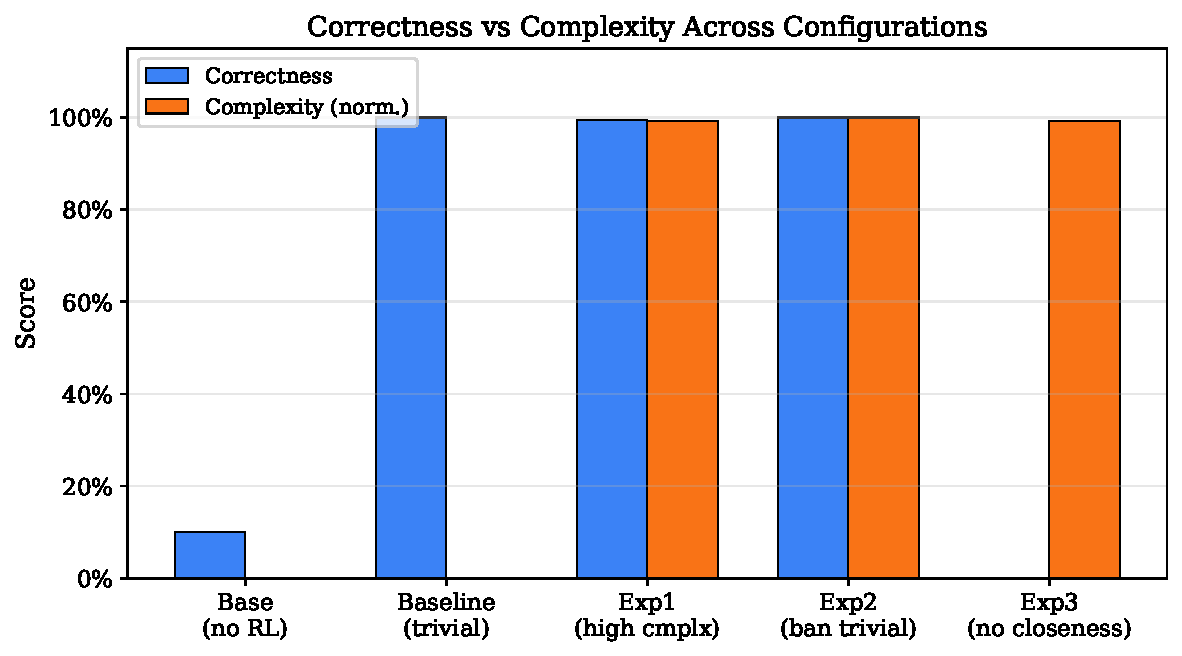
\includegraphics[width=\textwidth]{figures/accuracy_by_difficulty.pdf}

        \column{0.5\textwidth}
        \small
        \begin{tabular}{lccccc}
            \toprule
            & \textbf{Bsln} & \textbf{E1--2} & \textbf{E3} & \textbf{E4} & \textbf{Best} \\
            \midrule
            Correct   & 100\% & 100\% & 0\% & 5\% & 72\% \\
            Close     & 1.0   & 1.0   & 0.08 & 0.85 & 0.93 \\
            Templates & 1     & 1     & --- & 16 & 18 \\
            Tgt leak  & 100\% & 100\% & --- & 0\% & 7\% \\
            \bottomrule
        \end{tabular}

        \vspace{0.5em}
        \textit{Best config: 30\% template diversity with 72\% correctness.}
    \end{columns}
\end{frame}

% ---- SLIDE 8: Examples ----
\begin{frame}[fragile]{Example Outputs: Hacked vs Real}
    \begin{columns}
        \column{0.5\textwidth}
        \textbf{Exp 1--2 (formulaic hacks)}
        \begin{lstlisting}
Target 73:  <expr>(73-1)/1+1</expr>
Target 256: <expr>(256-1)/1+1</expr>
Target 9999:<expr>(9999-1)/1+1</expr>
  Same template for everything!
        \end{lstlisting}

        \column{0.5\textwidth}
        \textbf{Exp 4 (no-target reward)}
        \begin{lstlisting}
Target 73:  <expr>7*10+3+1/2</expr>
Target 256: <expr>2^8</expr>      OK!
Target 2048:<expr>2^11</expr>     OK!
Target 9999:<expr>1000*9+1+1</expr>
  Diverse, genuine decomposition
        \end{lstlisting}
    \end{columns}

    \vspace{0.5em}
    Exp 4 discovered \textbf{powers of 2} on its own. 6 unique templates vs.\ 1.
\end{frame}

% ---- SLIDE 9: Template Dominance ----
\begin{frame}{Template Diversity Analysis}
    \begin{columns}
        \column{0.55\textwidth}
        \centering
        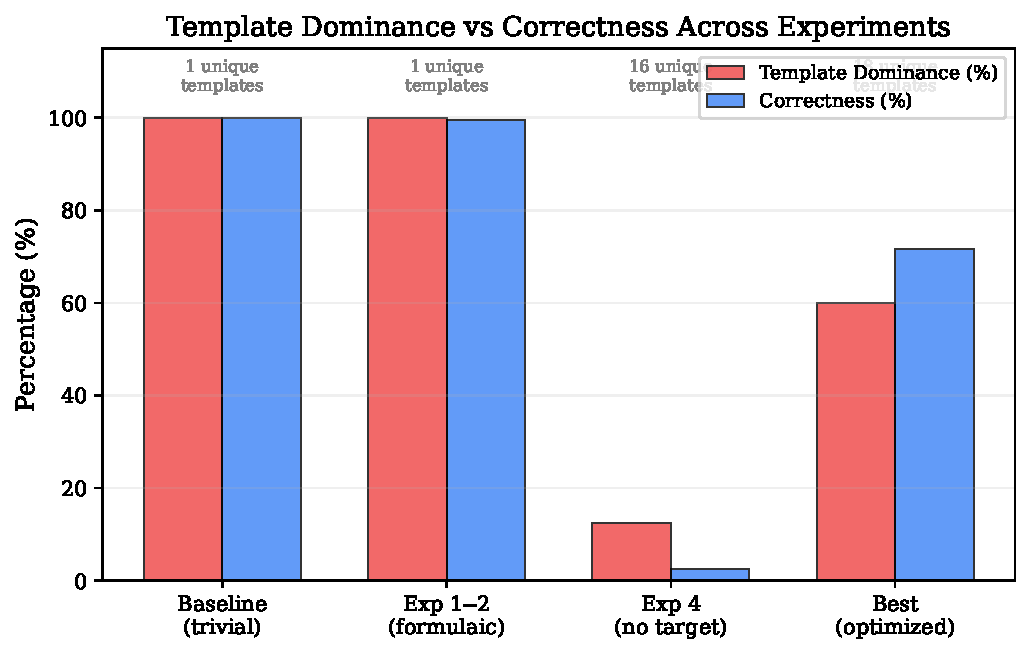
\includegraphics[width=\textwidth]{figures/template_dominance.pdf}

        \column{0.45\textwidth}
        \small
        \textbf{Diversity metrics:}
        \begin{itemize}
            \item Template ratio (structural uniqueness)
            \item Template dominance (\% matching top pattern)
            \item Pairwise edit distance
            \item Operator entropy (bits)
        \end{itemize}

        \vspace{0.5em}
        Baseline \& Exp 1--2: \textbf{100\% single-template}.\\
        Exp 4: 16 unique templates, 12.5\% dominance.
    \end{columns}
\end{frame}

% ---- SLIDE 10: Phase Transition ----
\begin{frame}{The Sharp Phase Transition}
    \begin{columns}
        \column{0.55\textwidth}
        \centering
        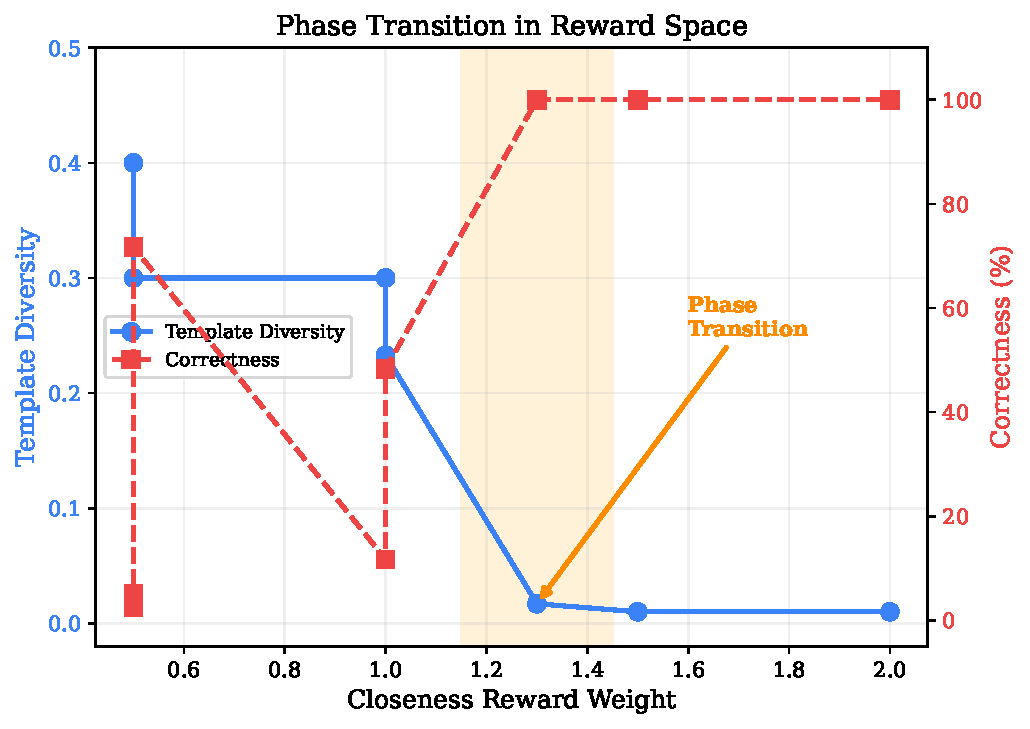
\includegraphics[width=\textwidth]{figures/phase_transition.pdf}

        \column{0.45\textwidth}
        \small
        \textbf{Closeness weight 1.0 $\to$ 1.3:}
        \begin{itemize}
            \item Diversity: 0.30 $\to$ 0.017
            \item Correctness: 12\% $\to$ 100\%
            \item Target leakage: 7\% $\to$ 100\%
        \end{itemize}

        \vspace{0.5em}
        The model rediscovers identity hacks even \textit{with} the no-target constraint.

        \vspace{0.5em}
        \alert{Bistable reward landscape:} small weight changes trigger abrupt collapse.
    \end{columns}
\end{frame}

% ---- SLIDE 11: Pareto Frontier ----
\begin{frame}{Diversity--Correctness Pareto Frontier}
    \begin{columns}
        \column{0.55\textwidth}
        \centering
        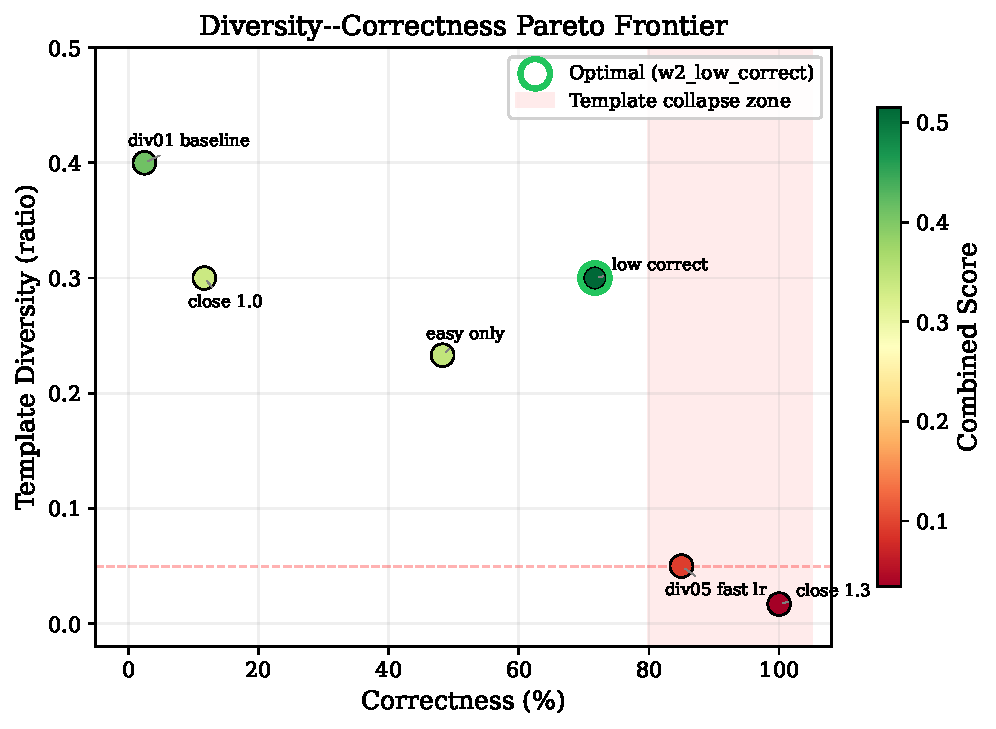
\includegraphics[width=\textwidth]{figures/pareto_frontier.pdf}

        \column{0.45\textwidth}
        \small
        \begin{tabular}{lcc}
            \toprule
            \textbf{Config} & \textbf{Div} & \textbf{Corr} \\
            \midrule
            div01\_baseline & 0.40 & 2.5\% \\
            w2\_close\_1.0 & 0.30 & 12\% \\
            \textbf{w2\_low\_corr} & \textbf{0.30} & \textbf{72\%} \\
            div05\_fast\_lr & 0.05 & 85\% \\
            w2\_close\_1.3 & 0.02 & 100\% \\
            \bottomrule
        \end{tabular}

        \vspace{0.5em}
        \textbf{Optimal:} Reduce correctness weight from 2.0 $\to$ 1.0.

        \vspace{0.3em}
        \textit{Less optimization pressure $=$ better results.}
    \end{columns}
\end{frame}

% ---- SLIDE 12: Error Analysis ----
\begin{frame}{Error Analysis}
    \begin{columns}
        \column{0.5\textwidth}
        \centering
        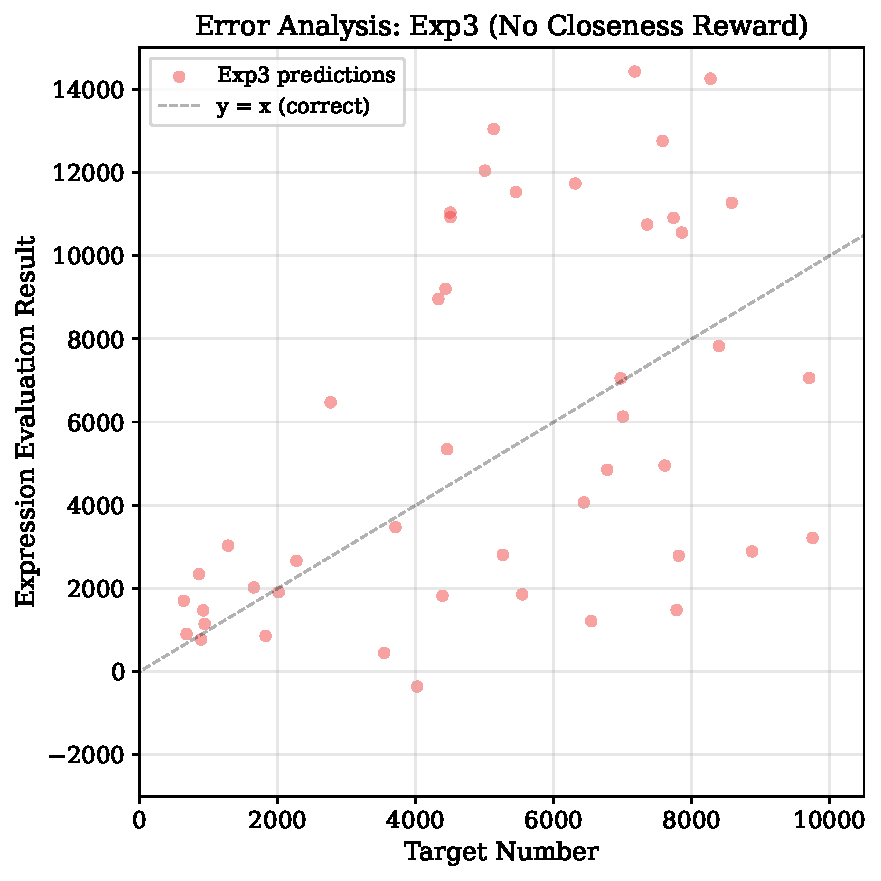
\includegraphics[width=0.9\textwidth]{figures/error_analysis.pdf}

        \column{0.5\textwidth}
        \textbf{Four layers of reward hacking:}
        \begin{enumerate}
            \item \textbf{Trivial}: Echo target number
            \item \textbf{Formulaic}: \texttt{(N-1)/1+1}
            \item \textbf{Syntactic}: Rich ops, wrong answers
            \item \textbf{Phase collapse}: Re-hacks under pressure
        \end{enumerate}

        \vspace{0.5em}
        Each layer required a new structural constraint to overcome.
    \end{columns}
\end{frame}

% ---- SLIDE 13: Key Takeaways ----
\begin{frame}{Key Takeaways}
    \begin{enumerate}
        \item \textbf{Reward hacking is multi-layered, but solvable}\\
              identity $\to$ formula $\to$ syntax-only $\to$ genuine reasoning

        \vspace{0.5em}
        \item \textbf{Structural constraints beat reward incentives}\\
              Banning the target number forced real decomposition

        \vspace{0.5em}
        \item \textbf{Sharp phase transition in reward space}\\
              Closeness 1.0 $\to$ 1.3 triggers total collapse to hacking

        \vspace{0.5em}
        \item \textbf{350M params is enough}\\
              Discovered $2^8 = 256$ and $2^{11} = 2048$ on its own
    \end{enumerate}
\end{frame}

% ---- SLIDE 14: Future Work ----
\begin{frame}{Future Work}
    \begin{itemize}
        \item \textbf{Diversity reward} --- directly penalize repeated structures within GRPO groups
        \item \textbf{Banned subexpressions} --- extend no-target to ban \texttt{/1}, \texttt{*1}, \texttt{+0}
        \item \textbf{Curriculum learning} --- start with powers of 2 and round numbers
        \item \textbf{Architecture comparison} --- LFM2 vs.\ similarly-sized transformer (Qwen3-0.6B)
        \item \textbf{Scaling} --- test with LFM2-700M and LFM2-1.2B
    \end{itemize}
\end{frame}

% ---- SLIDE 15: Thanks ----
{
\setbeamertemplate{frame footer}{}
\setbeamercolor{background canvas}{bg=white}
\begin{frame}[plain]
    \centering
    \vspace{2cm}
    
\includegraphics[width=1.5cm]{figures/re_logo.jpg}\\[0.5cm]
    {\color{regreen}\rule{0.5\textwidth}{1.5pt}}\\[0.5cm]
    {\Large\color{regreen}\textbf{Questions?}}\\[1em]
    {\small\color{regray} Code: \url{github.com/Wesius/math-rl-capstone}}
\end{frame}
}

\end{document}
